\chapter{Résultats et discussion}

\section{Données}
Dans cette section, nous allons décrire les pré-traitement sur les données (images) et mentionner leur source ainsi que le mode d'accès.
\subsection{Source et nature de données}

\subsubsection{SDSS(Sloan Digital Sky Survey IV)}
En termes simples, le Sloan Digital Sky Survey est l'étude astronomique la plus ambitieuse jamais entreprise. SDSS a observé en détail un quart de l'ensemble du ciel, déterminant les positions et la luminosité absolue de centaines de millions d'objets célestes\cite{sdss}. Il mesure également les distances à plus d'un million de galaxies et quasars\footnote{http://skyserver.sdss.org/dr13/en/sdss/sdsshome.aspx}. 

\subsubsection{DR13 (database release version 13)} \footnote{http://skyserver.sdss.org/dr13/en/help/browser/browser.aspx}
Data Release 13 stocke les prèmieres données de la quatièmes phase de la collecte de SDSS. Elle inclut les données prises à partir du 25 juin 2015, et englobe plus que un tiers de la sphère céleste. Avec plusieurs mesures du ciel faites et dans plusieurs façons, $1 231 051 050$ objets (catalogues) ont été collectés \footnote{http://www.sdss.org/dr13/scope/} 

\begin{figure}[H]
    \centering
    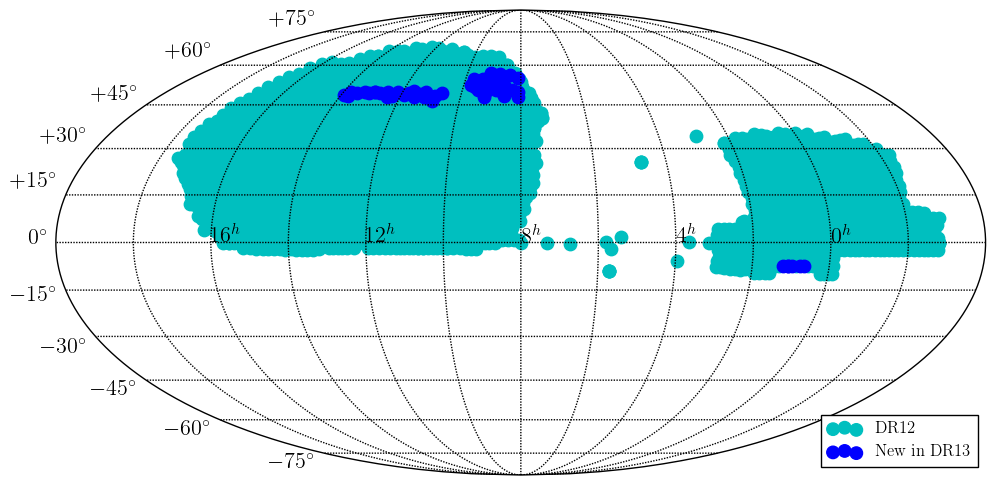
\includegraphics[scale = 0.5]{images/dr13_boss.png}
    %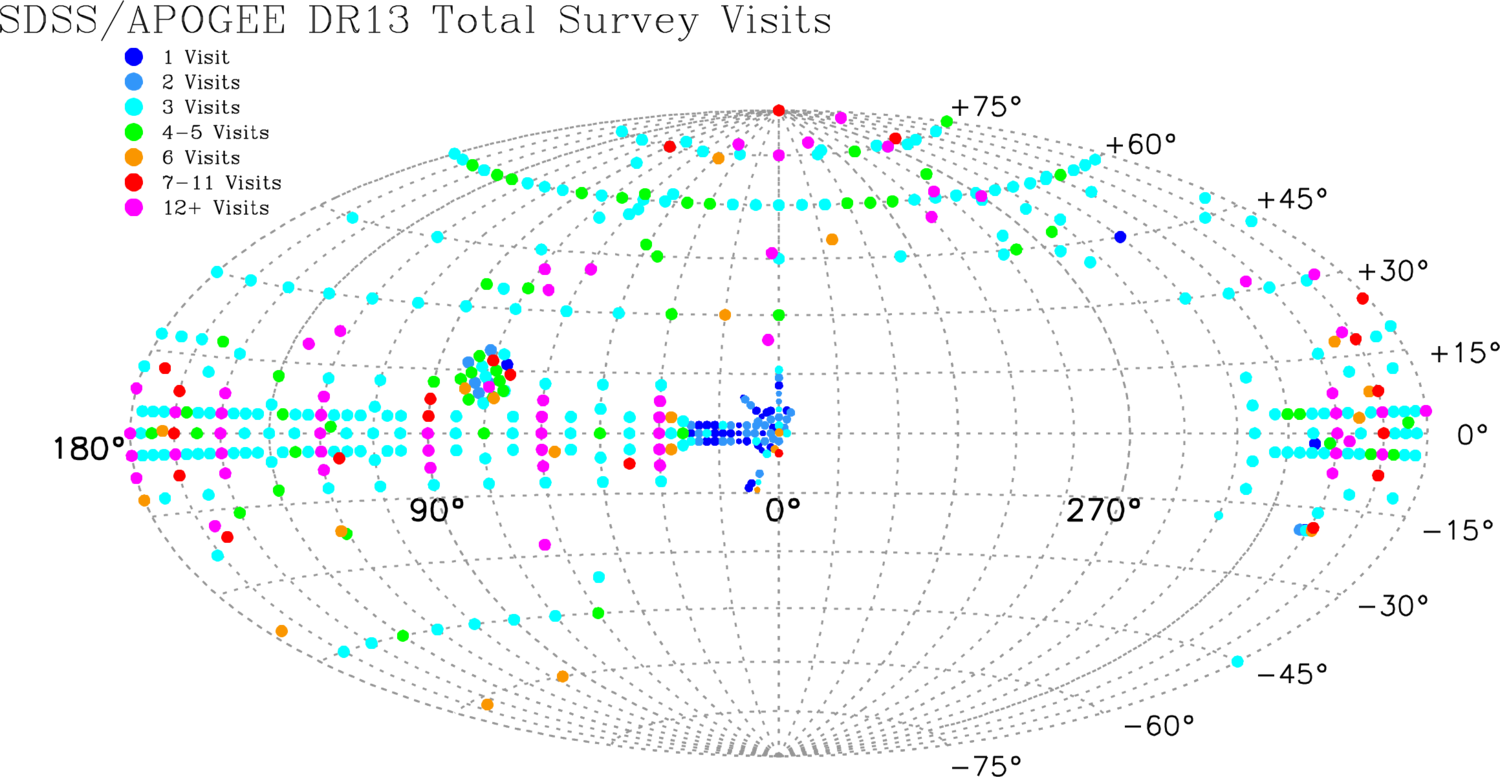
\includegraphics[scale = 0.3]{images/appoge.png}
    %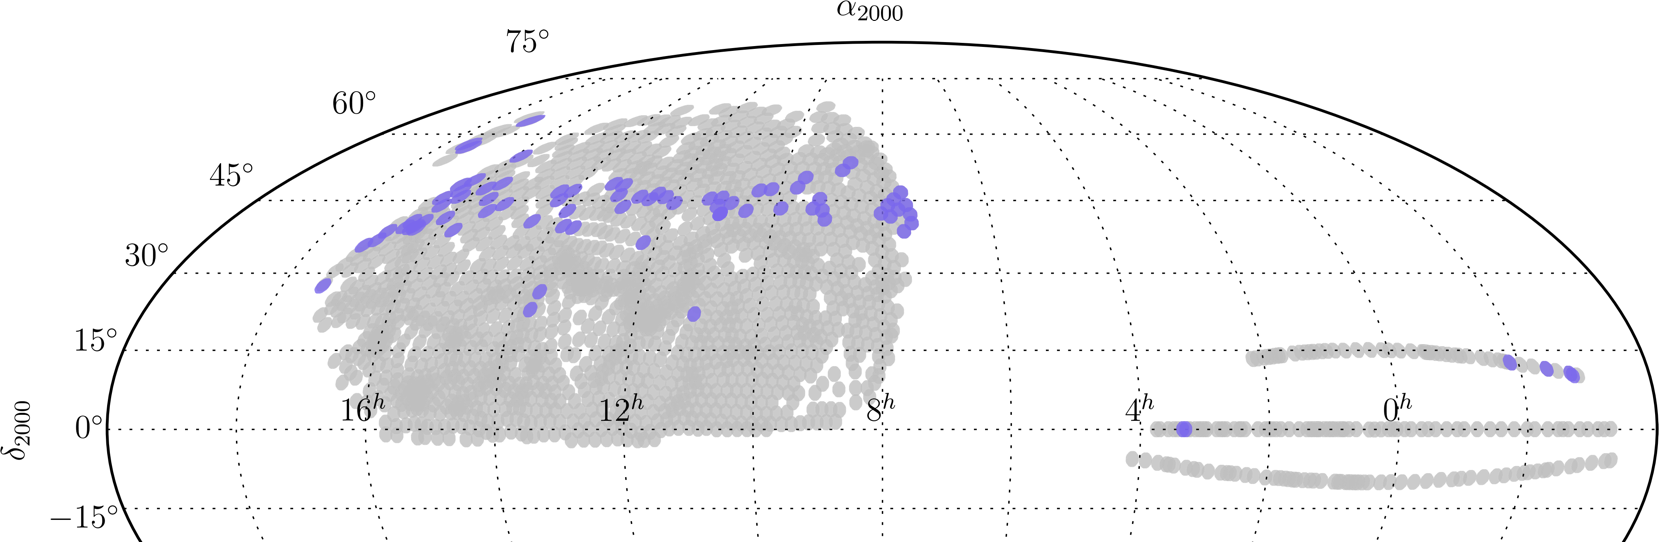
\includegraphics[scale = 0.1]{images/manga.png}
    \caption{eBOSS surveys}%, APOGEE surveys, and MaNGA surveys respectivement de gauche vers droite}
\end{figure}

Toutes nos données proviennent de la collecte de données SDSS . Elles sont télé-chargées sous forme des vecteurs chacune dans 5 bandes différentes (griuz). À partir de ces données sous forme de vecteurs provenant des tables SpecPhoto et PhotoPrimary de DR13 de SDSS, les urls des images correspondant à chaque vecteur sont générés. À partir de ces urls, les images sont télé-chargées et sauvegardées localement. \\

Les données ne sont pas sélectionnées, elles sont chargées directement aleatoires et sont de distributions différentes.
\begin{figure}[H]
	\centering
	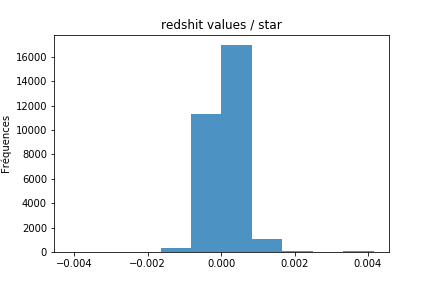
\includegraphics[scale = 0.3]{images/star.png}
	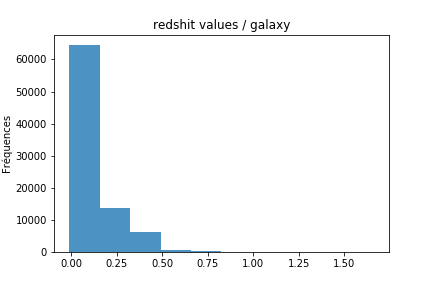
\includegraphics[scale = 0.3]{images/galaxy.png}
	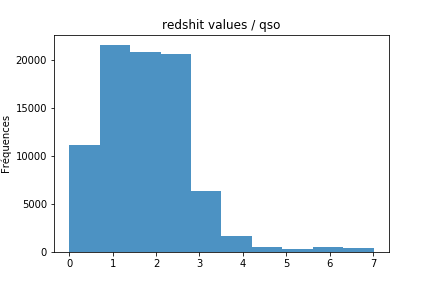
\includegraphics[scale = 0.3]{images/qso.png}
	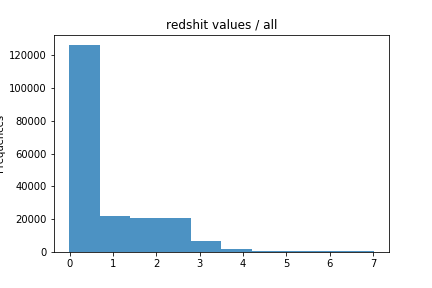
\includegraphics[scale = 0.3]{images/all.png}
	\caption{Distribution du redshift selon les catégories des objets cosmologiques}%, APOGEE surveys, and MaNGA surveys respectivement de gauche vers droite}
\end{figure}

\subsection{Pré-traitement sur les images}
Les images dans leur taille d'origine sont très grandes (1361*2048 pixels), et contiennent des quantités lumineuses très variées.
La taille de chaque image est réduite à 32*32, cette réduction est faite en utilisant la moyenne des coordonnées centrales (rowc$\_$ et colc$\_$) des objets(images) de chaque bande. Pour normaliser, le minimum de la quantité lumineuse (pixel) de chaque image est soustraite de l'image et le logarithme est appliqué à chaque pixel de l'image.  


\begin{figure}[H]
    \centering
    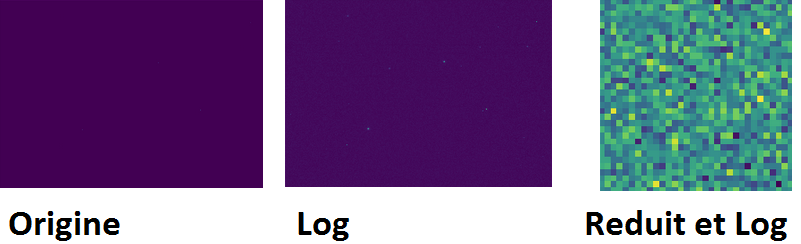
\includegraphics[scale = 0.5]{images/pretaitemen.png}
    \caption{pretement sur les images}
\end{figure}

\section{Configurations techniques}
Pendant toutes nos expérimentations, nous avons utilisés des machines hpc (haute performance computing) équipées d'une carte graphique graphique du type  NVIDIA GP104GL et un processeurs de 10 cœurs physiques de type Intel(R) Xeon(R) CPU E5-2640 v4 avec une fréquence de 2.40GHz.

Pour la concrétisation de notre architecture du CNN, nous avons utilisé la bibliothèque Keras \cite{chollet2015keras}  et pour celle du boosting nous avons utilisé la bibliothèque xgboost \footnote{http://xgboost.readthedocs.io} et scikit-learn \cite{scikit-learn}.
\section{Expérimentations}
Dans ce travail, nous avons choisi d'utiliser deux principales modèles de l'apprentissage automatique à savoir boosting qui est un modèle ensembliste, et réseau de neurones convolutifs (apprentissage profonds). En effets le boosting et les réseaux convolutifs ont donnée des bons résultats non pas seulement sur l'estimation du redshift \cite{meuphirim, isanto} mais également sur d'autres problèmes de régression et classification \cite{boost, adavencedCNN}. \\

Le choix et l'adaptation des hyper-paramètres ont été fait manuellement pour les deux types de modèles en faisant des test sur un petit échantillon de données et quelques combinaisons des hyper-paramètres. Au niveau du CNN, l'obtention des bons hyper-paramètres est compliquée car le CNN possède beaucoup d'hyper-paramètres à adapter.

Dans le tableau tab. \ref{quantite} est mentionnée la taille de données d'apprentissage et test de chaque type de corps cosmologiques.
\begin{table}[H]
	\centering
	\begin{tabular}{|l|l|l|}
		\hline
		$Type\_cosmologique$ & $\#Apprentissage$ & $\#Test$\\
		\hline
		Galaxie &  59887 & 25667\\
		\hline
		Quasar & 58668 & 25144\\
		\hline
		Étoile & 20994 & 8998 \\
		\hline
		Tous & 139550 & 59808 \\
		\hline
		%\hline		
	\end{tabular}
	\caption{Nombre d'élément de chaque type cosmologique}
	\label{quantite}
\end{table}


\subsection{CNN (type: inception module)}
Notre modèle final du type de réseau de neurones, celui qui s'adapte bien à nos données c'est-à-dire qui réduit mieux l'erreur normalisée ($\Delta z_{norm}$) est un réseau convolutif de la famille des inceptions modules. Notre modèle est construit comme suit: \\ Notre couche principale ($cp$) fig.\ref{archi_neural} est constituée de la concaténation de trois sous couches suivies par une sous couche d'agrégation de filtre 2 par 2 et d'un pas de déplacement 2 (strides = 2). Les trois sous couches concaténées sont décrites comme suit:
\begin{itemize}
	\item[$1^{er}$.] Constitué de trois sous couches de convolution de filtre 1*1 et de pas déplacement 1*1 formées de manière séquentielle.
	\item[$2^e$] Trois sous couches de convolutions formées de manière séquentielle de 3*3 comme filtre et de 1*1 comme pas déplacement.
	\item[$3^e$] Trois sous couches de convolution formées de manière séquentielle de 5*5 comme filtre et de 1*1 comme pas déplacement.
\end{itemize} 
\begin{figure}[H]
	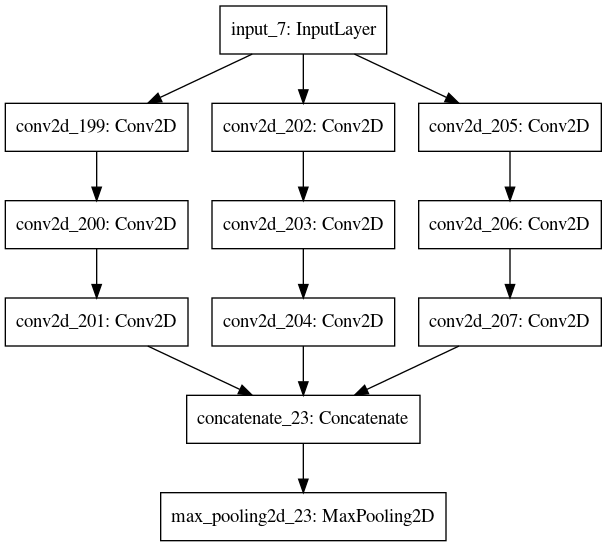
\includegraphics[scale = 0.5]{images/kernel.png}
	\caption{La couche principale de notre architecture neurale}
	\label{archi_neural}
\end{figure}
Dans chaque couche convolutive, la fonction d'activation est $relu(x) = max (0, x)$, pour éviter le sur-apprentissage une régularisation de type $l2$ est appliquée à chaque couche convolutive. Le padding zéro est appliqué sur toutes les couches convolutives. Notre architecture finale est constituée de 5 couches du même type que la $cp$ avec de nombre des sorties différents. Pour l'apprentissage, $Adam$ est utilisé entant qu'algorithme d'optimisation, à chaque deux reprises (epochs) de l'algorithme le taux d'apprentissage est divisé par deux, le early stoping est appliqué pour éviter le sur apprentissage de plus. Le early stoping est une manière d'arrêter rapidement l'apprentissage quand la précision sur les données d'apprentissage est sur le point de dépasser celle sur les données de validation. Le nombre de reprise(epochs) est paramétré à 30 et la taille de batch size est mise à 256.

Dans la suite du document, nous supposons les conventions suivantes:
$out1 = |znorm| > 0.15 (\%)$,  $out2 = |znorm| > 3std (\%)$, $RZ = RMSE\_znorm$ 
%\subsection{Expérimentions avec CNN}
\begin{table}[H]
	\centering
	\begin{tabular}{|l|l|l|l|l|l|l|}
		\hline
		type & $RZ$ & $\mu_{norm}$ & $\sigma_{norm}$ & RMSE & $out1$ & $out2$ \\
		\hline
		GXY/CNN & 0.035056 & 0.035032 & 0.035032 & 0.046099 & 0.752123 & 1.310150 \\
		\hline
		QSO/CNN & 0.289760 & 0.276163 & 0.276163 &1.065627 & 66.988385 & 0.441682\\
		\hline
		All/CNN & 0.261338 & 0.252728 & 0.252728 & 0.906072& 34.453168 &1.325543 \\
		\hline
		%\hline		
	\end{tabular}
	\caption{Résultats du CNN}
\end{table}

Ces résultats s'éloignent, dans le sens négatif, des meilleurs résultats de l'état de l'art. Cette mauvaise estimation de redshift par notre architecture de réseau convolutif peut s'expliquer par plusieurs raisons dont le fait qu'on possède moins de données pour booster l'apprentissage, le fait que l'image est trop réduite (trop de perte d'information) sans essayer de la réduire par la convolution.
 
\subsection{Boosting (type: xgboost)}
Trois principaux hyper-paramètres (nombre d'estimateurs, taux d'apprentissage et la profondeur de l'arbre) ont été réglés et adapté et tout le reste des paramètres ont été laissé avec leurs valeurs par défaut. Les trois modèles configurés du boosting sont mentionnés dans le tableau \ref{param_boost}.\\
\textbf{Quelques paramètres commun}\\
learning\_rate = 0.1, colsample\_bylevel=0.592, reg\_alpha=0.651, reg\_lambda=2.84
\begin{table}[H]
    \centering
    \begin{tabular}{|l|l|l|}
         \hline 
         modèles&n\_estimators&max\_depth\\
         \hline
          model1 &150&6\\
         \hline
         model3&150&5\\
         \hline         
         model2 &200&5\\
         \hline
         %mod1&&&&&&&
         %\hline
    \end{tabular}
    \caption{Paramètres de différents modèles de xgboost}
    \label{param_boost}
\end{table}

%\section{Résultats}


\subsection{Expérimentions avec XGBoost}
\begin{table}[H]
	\centering
	\begin{tabular}{|c|l|l|l|l|l|l|l|}
		\hline
		model & type & RMSE\_znorm & $\mu_{norm}$ & $\sigma_{norm}$ & RMSE & $out1$ & $out2$ \\
		\hline
		%\multirow{2}{1cm}{$model1$}& & & & & & \\
		
		\multirow{2}{1cm}{$model1$} & Galaxy  & 0.035728 & 0.000548 & 0.035723 & 0.046813 & 0.654537 & 1.137648 \\
		%\hline
		\cline{2-8}
		 & QSO & 0.318635  & 0.017468  & 0.318156  & 0.940743 & 64.03118 & 0.898823 \\
		 %\hline
		 \cline{2-8}
		 & All & 0.320223  & 0.015833  & 0.319832  & 0.801991 & 38.971375 & 2.543138 \\
		 %\hline
		 \cline{2-8}
		 & Star & 0.000429 & 0.000015  & 0.000428  & 0.000429 & 0.0       & 1.066904 \\
		 
		\hline
		\multirow{2}{1cm}{$model3$} & Galaxy  & 0.035938 & 0.000375 & 0.035936 & 0.04507 & 0.580512 & 1.133752 \\
		%\hline
		\cline{2-8}
		& QSO & 0.318635 & 0.017468 & 0.318156 & 0.940743 & 64.03118 & 0.898823 \\
		%\hline
		\cline{2-8}
		& All & 0.31818 & 0.010996 & 0.31799 & 0.799093	& 39.24057  & 2.539794 \\
		%\hline
		\cline{2-8}
		& Star & 0.000432 & 0.000013 & 0.000432 & 0.000433 & 0.0    & 1.044677 \\
		
		\hline
		\multirow{2}{1cm}{$model2$}& Galaxy & 0.03556 & 0.000058 & 0.03556 & 0.046432 & 0.654537 & 1.211673\\
		\cline{2-8}
		& QSO & 0.317182 & 0.016874 & 0.316733  & 0.957897	& 64.528317  & 	0.775533 \\
		\cline{2-8}
		& All & 0.320004 & 0.013142 & 0.319734 & 0.798689 & 39.569957 & 2.523074 \\
		\cline{2-8}
		&Star& 0.000423 & 0.000011 & 0.000423 & 0.000423 & 0.0 & 1.044677 \\
		\hline		
	\end{tabular}
	\caption{Résultats du XGBoost }	
\end{table}

Les résultats obtenus par xgboost sont intéressants et s'approchent mieux des ceux existants dans l'état de l'art \cite{meuphirim, isanto, photoredSDSS}. Nous remarquons que les modèles estiment bien les objets qui sont proches comme les étoiles puis les galaxies. Pour une estimation non biaisée tous les types de corps cosmologiques sont considérés et le modèle réduit mieux l'erreur sur l'ensemble de ces données fusionnées. 


















